\documentclass{article}
\usepackage{graphicx}
\begin{document}

%-------------------------------------------------------------------------------
%    TITLE PAGE
%-------------------------------------------------------------------------------

\begin{titlepage}
\newcommand{\HRule}{\rule{\linewidth}{0.5mm}}
\center
\textsc{\LARGE Imperial College London}  \\[1.5cm]
\textsc{\Large Department of Computing}  \\[0.5cm]
\textsc{\large Course 350: Management and Business for Computing Engineers} \\[0.5cm]

\HRule \\[0.6cm]
{\huge \bfseries name of company here} \\[0.3cm]
\HRule \\[1.5cm]

\begin{minipage}{0.4\textwidth}

% author
\begin{flushleft} \large \emph{Authors:} \\
Alina     \textsc{Boghiu}    \\
Giovanni  \textsc{Charles}   \\
Adam      \textsc{Fiksen}    \\
Sahil     \textsc{Jain}      \\
\L ukasz  \textsc{Koprowski} \\
Rutwick   \textsc{Shah}      \\
John      \textsc{Walker}    \\
\end{flushleft}

% supervisors
\end{minipage}~
\begin{minipage}{0.4\textwidth}

\begin{flushright} \large \emph{Lecturer:} \\
Nick \textsc{Coutts}
\end{flushright}


\end{minipage}\\[4cm]

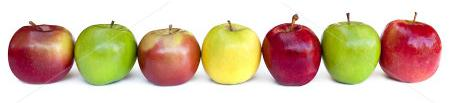
\includegraphics[width=\textwidth]{apples.jpg}

\end{titlepage}

%-------------------------------------------------------------------------------

\section{Executive summary}

business model = product (disguised as service for legal reasons - absolut?)

business objective 
maximise sales 
 - new to the market
   explain the required infrastructure to sell a lot 

\section{Vision statement}

%please discuss even if you do not think it is an issue
ethics - poverty, religion, corruption, age restriction, health, fairtrade,
eco(water recycling ...rutz..., using up all the apples)
%add as you please

%get the ethic vote, I think he really likes ethical companies
type = co-operative

\section{Management team}

\section{Introduction to the market}
\section{Products and services offered}
\section{Marketing plan}
 % summary of detailed plan including
	% prioritisation
	% validation
	% offers
	% routes to market

objective - maximise sales -> how

LTV = (Tn + ATV + LT) - (CoA + CoR) 
options which affect LTV

tailor LTV to get maximise value for target customer - guesswork market research
needs to be conducted

how this affects the supply chain
\section{Revenue model}
\section{Resource, cost and implementation plan}
revenue
 - retail
   licence
   other sales

profit
 - gross
   net
   EBITDA
   NPV

costs
 ...

sources of capital
 % Including headcount plan
\section{Product and systems development plans}
In order to setup a stable and longlasting infrastructure for our business we must take into consideration all the stages and requirements of production. This outlines a coherent development plan as follows.

	\begin{enumerate}
	\item Factory \\
When deciding about our homebase we considered two main criteria. The first regards our situation as a new company without assets. This brought the decision of renting out the factory bulding and equipment. The second criteria regards our main ingrediant requirements. Apples in India are available in the region of Himachal Pradesh. \\

For these reasons we will set our factory near Shimla, capital of Himachal Pradesh and rent the space and equipment necessary for production \\

\textbf{Quantities and Workforce} \\
For our marketing plan we require a relatively small production volume.\\
Workforce availability. \\

\textbf{Quality control}
We must ensure a good quality especially because it is a new product for this market..

	\item Suppliers
		\begin{itemize}
		\item Apple supply \\
			Buy from local farmers %who?
        	Sell residue back to farmers for animals (or agree on lower price)
		\item (Potentially) mango, berries, pares etc. suppliers
		\item Water supply \\
			Divine Waters, Foods Beverages
		\item Sugar supply %who?
		\item Bottling \\
			Home brewers use beer bottles, which work perfectly well, and are inexpensive. This allows the cider to become naturally carbonated.
		\end{itemize}
			
\item Risks \\
Eliminated some risk by:\\
	renting instead of building the factory\\
	buying instead of growing own apples\\
Workforce: lack of experience\\
Collaborators: \\
	\end{enumerate}


%1. how much money do we have
%2. how much can we do without partners
%3. where do we setup factories
%	what gets done in the factory
%4. where do we purchase equipment from
%5. who do we need to work for us
%6. distribution (how?)

\section{Capital requirements}
\section{Business opportunities and risks}
\section{Pro-forma financial projections}
\section{Risk analysis}

\end{document}
